\documentclass[a4paper]{article}
\usepackage[utf8]{inputenc}
\usepackage{amsmath}
\usepackage{amsfonts}
\usepackage{amssymb}
\usepackage{graphicx}
\usepackage{geometry}
\usepackage[english]{babel}
\usepackage{enumitem}%can be used for automatic numbering of requirements/tests.
\usepackage{hyperref}
\usepackage[colorinlistoftodos]{todonotes}
\usepackage{color} % Used to write in red,blue,green etc.
\usepackage{float}
\usepackage[titletoc]{appendix}

\newlength{\testlabellength}
\settowidth{\testlabellength}{Test 100.10.10}
\newenvironment{testlist}{\begin{enumerate}[label=\bfseries Test \thesubsection.\arabic* , labelindent=0pt, labelwidth=\testlabellength , leftmargin=2cm]}{\end{enumerate}}


\title{SVVS - Software Verification and Validation Specification}
\author{Testgroup, Team 2}


%-------------------------TITLE-----------------------------------------

\begin{document}
\begin{titlepage}
\newgeometry{left=2cm,top=1cm,right=2cm}
\newcommand{\HRule}{\rule{\linewidth}{0.5mm}}

\begin{minipage}{0.5\textwidth}
\begin{flushleft} % Responsible persons, write on separate lines
\textit{Responsible for this document:}\\
Oskar Fällström %Not entirely sure who this should be, possibly project leaders as well?
\end{flushleft}
\end{minipage}
~
\begin{minipage}{0.4\textwidth}
\begin{flushright}
PUSS154213 v0.1 %Dokumentnummer enl. projekthandledning s. 22-23 och insidan av pärmen
\today
\end{flushright}
\end{minipage}\\[3cm]

\centering
\textsc{\LARGE Team 2}\\[0.5cm]

\HRule \\[0.4cm]
{ \huge \bfseries Software Verification and Validation Specification}\\[0.4cm] % Title of your document
\HRule \\[1.5cm]

\vfill
\begin{flushleft}
\textit{Authors of this document:}\\
Måns Andersson \\
Hanna Autio \\
Moa Eklöf \\
Oskar Fällström \\
Ulf Hörndahl \\
Jonathan Lundholm
\end{flushleft}


\end{titlepage}
\pagenumbering{gobble}
\setcounter{tocdepth}{2}
\tableofcontents
\newpage
\pagenumbering{arabic}

%--------------------Introduction ---------------------------------------
\section{Introduction}
The Software Verification and Validation Specification (SVVS) describes all tests and reviews conducted during the development of the project. The document acts as a base for the SVVI (Software Verification and Validation Instruction).
In the main document, there are instructions for reviews as well as information about what types of tests should be performed and by whom. In the appendices, test cases are specified.

%--------------------Reference Documents ---------------------------------------
\section{Reference Documents}
\begin{enumerate}
\item PUSS154212 - System Requirements Specification for the current project \label{refdocs:srs}
\item Programvaruutveckling för stora system - Projekthandledning (\textit{Institutionen för datavetenskap}, Lunds Univeritet 2015) \label{refdocs:projekthandledning}
\end{enumerate}

%--------------------Definitions-------------------------------------------
\section{Definitions}
\begin{description}
\item[SDP] Software Development Plan
\item[SRS] Software Requirements Specification
\item[SVVS] Software Verification and Validation Specification
\item[SVVI] Software Verification and Validation Instruction
\item[STLDD] Software Top Level Design Document
\item[SDDD] Software Detailed Design Document
\item[SVVR] Software Verification and Validation Report
\item[SSD] Software Specification Document
\item[PFR] Project Final Report
\item[PG] Project Group Leaders
\end{description}
%--------------------Testing ---------------------------------------
\section{Testing}
In order to validate and verify that the system fulfills the customers expectations, various tests are conducted during the development phases. Types of test i.e. unit tests, function tests etc. can be divided into two categories: white-box tests and black-box tests, which are described below. Both of these should be performed.  

\subsection{White-box Testing}
In a white-box test the developer tests the internal structure of the system, by means of making sure that all lines/units of code are executed at least once. These are performed by the developer group during development.

\subsection{Black-box Testing}
A function test or black-box test examines the functionality of a system from an external point of view. Combinations of input data are chosen and the output data from the system is compared to a specification.


%--------------------Reviews ---------------------------------------
\section{Reviews}

\subsection{Formal Reviews}
Formal reviews are conducted according to reference \ref{refdocs:projekthandledning}.

The scheduled formal reviews, and the documents up for review, in this project are:

\begin{enumerate}

\item Software Specification Review (SSR)
\begin{itemize}
\item SDP
\item SRS
\item SVVS
\end{itemize}


\item Preliminary Design Review (PDR)
\begin{itemize}
\item SVVI
\item STLDD
\end{itemize}


\item Product Review (PR)
\begin{itemize}
\item SVVR
\item SSD
\item PFR
\end{itemize}


\end{enumerate}


\subsection{Informal Reviews}
Informal reviews are to be held before the deadline for the formal review, with enough time to correct any problems found during the informal review. The documents up for review should be made available in the project library at least 24 hours before the informal review.

PG are the responsible coordinators for the informal review.

%--------------------Test environments ---------------------------------------
\section{Test Environments}
All tests specified in this document should be performed on appropriate emulator software. If possible, the tests should also be run on a physical device.

%--------------------Test cases ----------------------------------------------
\section{Types of Tests}

\subsection{Unit Tests}
The developer group should perform unit tests, both black-box tests and white-box tests. These tests should be performed continuously during development.

\subsection{Function Tests}
All functions of the system should be tested according to appendix \ref{appendix:section:functiontest}. The test group is responsible for  performing these tests.

\subsection{System Tests}
The entire system should be tested according to appendix \ref{appendix:section:systemtest}. The test group is responsible for performing these tests. 

\subsection{Regression Tests}
After any changes, all system tests should be performed again to ensure that previously functional code is still working. The test group is responsible for performing these tests.

\subsection{Acceptance Tests}
Acceptance tests are performed by the costumer before completion of the project. The costumer is responsible for selecting tests to ensure that the software meets their demands.

%--------------------Appendix A: Function test Specification ----------------
\newpage
\begin{appendices}

\section{Function Test Specification} \label{appendix:section:functiontest}
This is appendix A where we list all function test specifications.

\subsection{MyDevices View Tests}
\begin{testlist}
	\item The list of available devices is empty on application start up. (Req. 5.2.2)
    \item The list on the MyDevices view is scrollable. (Req. 5.2.3)
   
    \item The items on the list are selectable. (Req 5.2.4)
    \item Only one device can be selected at a time. (Req. 5.2.5)
    \item When no device is selected and the "Control Device" -button is pressed, a pop-up message "Please select device" is displayed. (Req. 5.2.6)
    \item Sensors are displayed in the list of available devices with "Sensor" as name, and it's MAC address as address. (Req. 5.2.7)
    \item Light bulbs are displayed in the list of available devices with "Light Bulb" as name and it's MAC address as address. (Req. 5.2.8)
    \item The "Get Devices" -button performs a scan for available devices when pressed. (Req. 5.2.9)
    \item When the back button is pressed the application is closed (Req. 5.2.10)
\end{testlist}

%--------------------------Sensor view tests --------------------------------------
\subsection{Sensor View Tests}
\begin{testlist}
\item When the "Control Device"-button in the MyDevices View is pressed and a sensor is selected, the Sensor view is opened. (Req. 5.3.1)

\item The sensor name and mac-address is shown in the top of the view (Req. 5.3.2, 5.3.3)
 
\item It is possible to change the on/off -status of the selected sensor with a switch. (Req. 5.3.4)

\item There are text fields preceded by "T", "P", "H", "M", "G", "A" that are used to, respectively, display temperature, pressure, humidity, magnetic field, gyroscopic value and acceleration. (Req. 5.3.5, 5.3.6, 5.3.7, 5.3.8, 5.3.9, 5.3.10)

\item By pressing the corresponding "Get"-button, the values of the temperature, pressure, humidity, magnetic field, qyroscopic and acceleration sensors are retrieved if available and displayed. (Req. 5.3.11, 5.3.12, 5.3.13, 5.3.14, 5.3.15, 5.3.16)

\item The "Get all" -button gets the values for all available sensors and displays them.(Req. 5.3.17)
\item The "clear-all" button clears all sensor text fields from data. (Req. 5.3.18)
\item If there is no data to retrieve for any of the physical quantities temperature, pressure, humidity, magnetic field, gyroscopic and acceleration when the corresponding "Get" button is pressed the corresponding text fields display "No data available".(Req. 5.3.19, 5.3.20, 5.3.21, 5.3.22, 5.3.23, 5.3.24)

\item The on/off-switch is set according to the information from the REST API. (5.3.25)

\item When the sensor view is opened the temperature, pressure, humidity, magnetic field, gyroscopic and acceleration text fields are empty. (Req. 5.3.27)

\end{testlist}

\subsection{Lightbulb View}
\begin{testlist}
	\item The Light Bulb View opens when a light bulb is chosen in the MyDevices View and the "Select device" button is pressed. (Req 5.4.1)
	\item The name of the selected light bulb is shown in the top of the View. (Req 5.4.2)
  
    \item The state of the selected light bulb can be changed with a switch. (Req. 5.4.3)
    
    \item The field of R-, G-, B-, W-value is editable and preceded by "R:", "G:", "B:" and "W:" respectively. (Req. 5.4.4, 5.4.5, 5.4.6, 5.4.7) 

    
	\item When the Light Bulb View is opened, the fields are empty. (Req. 5.4.8)

	\item The "Get"-button receives the R-, G-, B-, W-values and present them in the fields specified in requirement 5.4.4 to 5.4.7. (Req. 5.4.9)

	\item The "Set button" sets the color of the light bulb.	(Req. 5.4.10)

	\item If an input value is left blank the value is interpreted as 00. (Req. 5.4.11)    
    
    
    \item The value representing the color of the fields is of maximum two characters. (Req. 5.4.12)
    
    \item The fields only accepts two characters that represent hexadecimal numbers (e.g. 00 to FF and all combinations inbetween). (Req 5.4.12, Req 5.4.13)
    
    \item A pop-up message saying "Color successfully changed" is displayed when the values of the light bulb were successfully set. (Req 5.4.14)
    
    \item The application checks the input values when the "Set"-button is pressed. If the values are out the specified range, a pop-up message is displayed saying: "Input values out of range" (Req 5.4.13 and Req 5.4.15)
    
    \item When the light bulb is off, the "Set"-button is unavailable. (Req. 5.4.16)
    
    \item When the back button is pressed the system switches to My Devices View. (Req. 5.4.17)

\end{testlist}	

%--------------------Appendix B: System test Specification ----------------
\newpage

\section{System Test Specification} \label{appendix:section:systemtest}
This is appendix B where we list all system test specifications.

\subsection{Use Cases}
\begin{testlist}
	\item Use case 5.1.1 in Ref \ref{refdocs:srs} is supported. (Req. 5.1.1)
	\item The exception described in use case 5.1.1 can be generated by removing the devices from range while attempting use case 5.1.1. (Req 5.1.1)
	
	\item Use case 5.1.2 in Ref \ref{refdocs:srs} is supported. (Req. 5.1.2)
	
	\item The exception in use case 5.1.2 can be generated by not selecting a device in step 1. (Req. 5.1.2)
	
	\item Use case 5.1.3 in Ref \ref{refdocs:srs} is supported. (Req. 5.1.3)
	
	\item The exception described in use case 5.1.3 can be generated by not selecting a device in step 1. (Req. 5.1.3)
	
	\item Use case 5.1.4 in Ref \ref{refdocs:srs} is supported. (Req. 5.1.4)
	
	\item Use case 5.1.5 in Ref \ref{refdocs:srs} is supported. (Req. 5.1.5)
	
	\item Use case 5.1.6 in Ref \ref{refdocs:srs} is supported. (Req. 5.1.6)
	
	\item Use case 5.1.7 in Ref \ref{refdocs:srs} is supported. (Req. 5.1.7)
	
	\item Use case 5.1.8 in ref \ref{refdocs:srs} is supported. (Req. 5.1.8)
	
	\item A popup message reading "Fill in all fields" can be generated by not entering any data into some of the colour fields when attempting use case 5.1.8. (Req. 5.1.8)
	
	\item Use case 5.1.9 in Ref \ref{refdocs:srs} is supported. (Req. 5.1.9)
	
	\item If some data is unavailable when attempting use case 5.1.9, the text in the corresponding field is set to "No data available." (Req. 5.1.9)
	
	\item Use case 5.1.10 in Ref \ref{refdocs:srs} is supported. (Req. 5.1.10)
	
	\item If some data is unavailable when attempting use case 5.1.10, the text in the corresponding field is set to "No data available." (Req. 5.1.10)
	
	\item Use case 5.1.11 in Ref \ref{refdocs:srs} is supported. (Req. 5.1.11)
	
	\item If some data is unavailable when attempting use case 5.1.11, the text in the corresponding field is set to "No data available." (Req. 5.1.11)
	
	\item Use case 5.1.12 in Ref \ref{refdocs:srs} is supported. (Req. 5.1.12)
\end{testlist}

\subsection{Appearance and Layout}

\begin{testlist}
	\item The first screen that is shown on startup is the MyDevicesView. (Req. 5.2.1)
	
	\item When the back button is pressed in the MyDevices View, the application is closed. (Req. 5.2.10)	
	
	\item When the back button is pressed in the Sensor View, the MyDevices View is opened. (Req. 5.3.26)
	
	\item When the back button is pressed in the Light Bulb View, the MyDevices View is opened. (Req. 5.4.17)
	
	\item The layout of the MyDevices View resembles figure 1 in reference \ref{refdocs:srs} (Req. 6.1).
	
	\item The layout of the Sensor View resembles figure 2 in reference \ref{refdocs:srs} (Req. 6.2).
	
	\item The layout of the Light Bulb View resembles figure 3 in reference \ref{refdocs:srs} (Req. 6.3).
	
	\item Test of usability using persons without prior knowledge of the project or the app. (Req. 6.4)
\end{testlist}

\clearpage
\section{Test Matrices}
\begin{figure}[H]
    \centering
    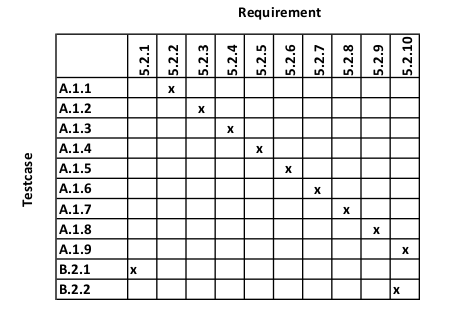
\includegraphics[scale=0.9]{SVVS-pics/testmatrixMyDevices.png}
    \caption{Test matrix for The My Devices View.}
    \label{fig:testmatrix-mydevices}
\end{figure}

\begin{figure}[H]
    \centering
    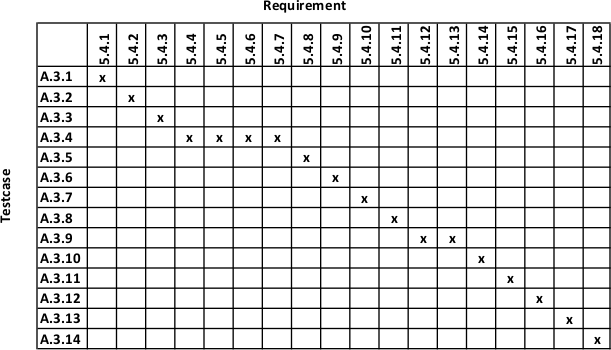
\includegraphics[scale=0.9]{SVVS-pics/testmatrixLightbulb.png}
    \caption{Test matrix for The Lightbulb View.}
    \label{fig:testmatrix-lightbulb}
\end{figure}

\begin{figure}[H]
    \centering
    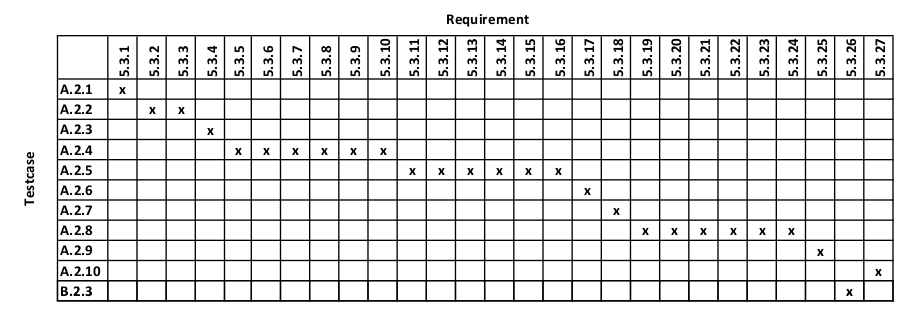
\includegraphics[scale=0.9,angle=-90]{SVVS-pics/testmatrixSensor.png}
    \caption{Test matrix for The Sensor View.}
    \label{fig:testmatrix-sensor}
\end{figure}

\begin{figure}[H]
    \centering
    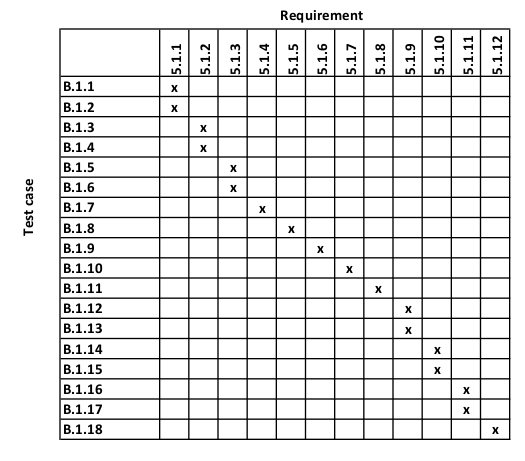
\includegraphics[scale=0.9]{SVVS-pics/testmatrixUsecases.png}
    \caption{Test matrix for the use cases.}
    \label{fig:testmatrix-usecase}
\end{figure}

\begin{figure}[H]
    \centering
    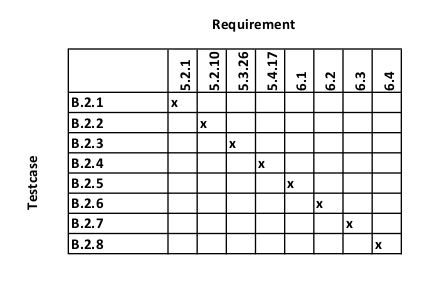
\includegraphics[scale=0.9]{SVVS-pics/testmatrixLayout.png}
    \caption{Test matrix for the layout.}
    \label{fig:testmatrix-layout}
\end{figure}
\end{appendices}


\end{document}